% !TEX root =  master.tex
\chapter{Theoretische Grundlagen}
\section{Moderne Technologien und Softwarekonzepte}
\subsection{Software-as-a-Service}
\label{theorie_saas}
Bei \acl{SaaS} handelt es sich um einen angebotenen Dienst, der dem Benutzer die Installation und den Betrieb der Software vollständig abnimmt und diese beispielsweise mittels einer Webanwendung auf dem höchstmöglichsten Abstraktionslevel bereitstellt. Dabei sollte im Optimalfall die gleiche Funktionalität wie in einer konventionellen Desktopanwendung abgedeckt werden. 
\autocite[Vgl.][S. 13, 15]{Buyya.2011} \\
Grundlage für \ac{SaaS} ist das Konzept des \textbf{Cloud Computings}. Cloud Computing basiert auf dem \textbf{Grid Computing}, welches verteilte und voneinander unabhängige Ressourcen, wie zum Beispiel \acsp{CPU}, Arbeitsspeicher und Speicherplatz virtuell aggregiert und dem Benutzer als ein einziges System darstellt. Spezifisch bedeutet Cloud Computing jedoch, dass die durch Grid Computing virtualisierten Rechenressourcen \textbf{as-a-Service} für Unternehmen und Endverbraucher angeboten werden.\\
Zudem ermöglicht Cloud Computing die Entwicklung von geographisch unabhängigen Anwendungen, welche abhängig vom Rechenbedarf dynamisch skaliert werden können.\autocite[Vgl.][S. 3]{Buyya.2011}\\
Innerhalb des Cloud Computings hat sich laut James Broberg das sogenannte \textbf{Pay-Per-Usage}-Kostenmodell etabliert, bei dem der Benutzer des Cloud Computing Dienstes ausschließlich für die effektiv genutzten Rechenressourcen bezahlen muss.\autocite[Vgl.][S. 9-10]{Buyya.2011}\\
Im Bereich des Cloud Computings haben sich besonders die Hyperscaler durchgesetzt, die laut einer Studie der ISG Information Services Group aus dem Jahr 2018 fast zwei Drittel des deutschen Cloud Computing Marktes eingenommen haben.\autocite[Vgl.][S. 1]{Henkes.2018}\\
Dazu gehören unter anderem \ac{AWS}, Google mit der \ac{GCP} und Microsoft Azure. Diese zielen besonders auf die dynamische und regionale Skalierbarkeit der Infrastruktur ab, mit der die Performance und regionale Verfügbarkeit optimiert werden kann.\\
Laut P. Mell und T. Grance, welche in ihrer ``The NIST definition of Cloud Computing`` im Jahre 20100 Cloud Computing definierten, kann Cloud Computing in drei Klassen unterteilt werden. Diese unterscheiden sich mittels des Abstraktionslevels der Dienste und dem Dienstleistungsmodell der Anbieter.\autocite[Vgl.][S. 2-3]{Mell.2011}\\
Jedoch ist diese Definition auf Grund der Weiterentwicklungen innerhalb der letzten Jahre kritisch zu betrachten, da sich die damals definierten Klassen: \ac{IaaS}, \ac{PaaS} und \ac{SaaS} mittlerweile angesichts neuer Softwarekonzepte und Technologien weiterentwickelt haben.\\
Erweitert wurde die Klassendefinition des Cloud Computings laut Oliver Liebel exemplarisch durch die Entwicklung der Containerisierung der Infrastruktur. Daraus entstanden zum Beispiel die weiteren Cloud Computing Klassen wie \textbf{Container-as-a-Service} oder \textbf{Function-as-a-Service}.\autocite[Vgl.][S. 55-56]{Liebel.2019} Bestätigt wird das as-a-Service Vertriebsmodell von Mario Meir-Huber, der bereits im Jahr 2011 von \textbf{Everything-as-a-Service} sprach, in dessen Richtung sich die Softwarebranche immer mehr entwickelt. \autocite[Vgl.][S. 32]{MeirHuber.2011}\\
Bei der wirtschaftlichen Betrachtung von \ac{SaaS}-Lösungen und der Partnerschaft mit \ac{IaaS}-Providern spielen besonders die schnelle Time-To-Market, die dynamische Skalierbarkeit und das Pay-per-Usage Kostenmodell eine wichtige Rolle. Insgesamt sollten bei der Investitionsrechnung jedoch immer die \ac{TCO} betrachtet werden, um einen korrekten Kostenvergleich mit beispielsweise einer On-Premise-Lösung durchführen zu können. Diese setzen sich unter anderem aus den einmaligen Kosten für die Softwarelizenz und den für den Wartungsservice anfallenden laufenden Kosten zusammen. \autocite[Vgl.][S. 63-66]{Metzger.2011}

\subsection{Microservices}
Microservices sind unter anderem im Zuge der Modularisierung großer monolithischer Softwarekomplexe in einzelne voneinander unabhängige Komponenten entstanden. Ziel der Aufteilung des monolithischen Komplexes ist es, die einzelnen Softwarekomponenten voneinander zu entkoppeln, um die Resilienz des Gesamtsystems verbessern zu können. Darunter wird die Widerstandsfähigkeit des Gesamtsystems bei einem Ausfall einzelner Systemkomponenten verstanden. Diese Widerstandsfähigkeit ist besonders bei verteilten Softwaresystemen relevant, um die durch eine verteilte Systemarchitektur erhöhte Wahrscheinlichkeit eines unkontrollierten Gesamtausfalles des Systems minimieren zu können.\autocite[Vgl.][S. 1-2]{Wagner.2016}\\
Hierfür werden die einzelnen Microservices als eigenständige Prozesse auf einer \ac{VM} ausgeführt. Für die Kommunikation der Microservices untereinander wird das gemeinsame Netzwerk und die darauf aufbauenden Netzwerkprotokolle, wie beispielsweise das \ac{HTTP}, verwendet. Dabei hat sich die asynchrone Kommunikation mittels eigener \ac{REST}-Schnittstellen oder auch Messaging-Lösungen, wie zum Beispiel RabbitMQ, etabliert. Durch die asynchrone Kommunikation wird die lose Kopplung der eigenständigen Software-Komponenten unterstützt.\autocite[Vgl.][S. 1-2, 64-65]{Wolff.2016} \\
Des Weiteren ist eine auf Microservices basierende Softwarearchitektur die essentielle Grundlage für die Entwicklung einer Cloud nativen \ac{SaaS}-Lösung. Dies begründet sich seitens der folgenden Aufzählung der Vorteile einer solchen Architektur, welche von Eberhard Wolff festgestellt wurden.
\begin{description}
\item[Einsatz unterschiedlicher Technologien] \hfill \\
Bei der Konzeption und Entwicklung der einzelnen Microservices können voneinander unabhängige Technologieentscheidungen getroffen werden. Dadurch können die Microservices beispielsweise in unterschiedlichen Programmiersprachen implementiert werden. Zudem ermöglicht die Microservice-Architektur die Umsetzung des \textbf{Database-per-Component}-Konzeptes. Dieses Konzept sieht den Einsatz der jeweils für den Microservice technologisch am besten geeigneten Datenbank vor. 
\item[Freie Skalierbarkeit der einzelnen Microservices] \hfill \\
Durch die voneinander unabhängige Bereitstellung der Microservices wird die Skalierung auf einzelner Microservices ermöglicht. Damit können zum Beispiel rechenintensive Softwarekomponenten auf leistungsstärkerer Hardware betrieben werden. 

\item[Unabhängige Versionierung] \hfill \\ 
Zusätzlich zur unabhängigen Skalierung kann auch die Versionierung der Microservices und deren Aktualisierungen voneinander getrennt durchgeführt werden. Jedoch sollte hierbei beachtet werden, dass es an der Funktionsweise der externen Schnittstelle keine ungeplanten Änderungen gibt und weiterhin die Abwärtskompatibilität bestehen bleibt.

\item[Continious Delivery] \hfill \\
Außerdem unterstützt eine auf Microservices basierende Architektur den \ac{CI}- und \ac{CD}-Ansatz von DevOps-Teams, da Anpassungen und Erweiterungen der einzelnen Microservices unabhängig von anderen Entwicklungsteams direkt implementiert und bereitgestellt werden können.

\item[Eindeutige Definition von Abhängigkeiten] \hfill \\
Da die Entwickler der Microservices für die Kommunikation mit anderen Microservices explizit die zur Verfügung gestellten Schnittstellen verwenden müssen, sind Abhängigkeiten eindeutig erkennbar und können beispielsweise nicht, wie bei monolithischen Architekturansätzen, durch unerwünschtes Wiederverwenden einer externen Klasse entstehen.\autocite[Vgl.][S. 3-5, 59-63]{Wolff.2016}
\end{description}
\newpage
Jedoch existieren neben den zuvor genannten Vorteilen einer Microservice-Architektur auch Nachteile.\\
Besonders die erhöhte Komplexität der Softwarearchitektur sollte bei der Entscheidung für eine Microservice-Architektur berücksichtigt werden. Des Weiteren kann die fachliche Aufteilung des Softwarekomplexes in einzelne Microservices besonders bei stark voneinander abhängigen Softwarekomponenten eine Herausforderung darstellen. Auch die Performance kann durch die zusätzlich benötigte Kommunikation der Microservices über das Netzwerk beeinträchtigt werden. Neben der Architektur der Software ist auch der Betrieb der auf Microservice basierenden Softwarelösung komplexer, da die Komponenten alle einzeln bereitgestellt, überwacht und verwaltet werden müssen. Zudem werden auch Mechanismen zur Sicherstellung der Konsistenz innerhalb der verteilten Softwarelösung benötigt.\autocite[Vgl.][S. 73-77]{Wolff.2016} \\
Die zuvor genannten generellen Herausforderungen bei der Verwendung von Microservices sind der Ursprung für die Entwicklung eines automatisierten Plattformbetriebs und der daraus entstandenen Container-Orchestrierungsplattform Kubernetes gewesen. Kubernetes bietet hierbei Lösungsansätze an, die beispielsweise auf dem Replizieren der einzelnen Softwarekomponenten basieren. Weitere Funktionsweisen und die Erläuterung des Aufbaus eines Kubernetes Clusters folgen im Kapitel \ref{Kubernetes}.\\
Generell sollte bei einer auf Microservice basierenden Architektur besonders das \ac{KISS}-Prinzip verfolgt werden. Dieses bedeutet im Microservice-Umfeld, dass nicht erzwungenermaßen aus jeder möglichen Applikationskomponente ein einzelner Microservice konzipiert werden sollte, da dies den Administrationsaufwand erhöht und auch die generelle Wartbarkeit der Softwarelösung auf Grund der Komplexität verschlechtert.\autocite[Vgl.][S. 60]{Liebel.2019} \\

\subsection{Cloud Foundry Plattform}
\acl{CF} ist eine Cloud native Anwendungsplattform. Die Besonderheit einer nativen Cloudplattform ist laut Duran Winn, dass diese trotz der Verwendung von potenziell unzuverlässiger Cloud-Infrastruktur eine zuverlässige und skalierbare Bereitstellung von Anwendungen ermöglicht.\autocite[Vgl.][S. 1]{Winn.2017}\\
Dies wird durch zusätzliche Mechanismen, welche bei nicht Cloud nativen Anwendungsplattformen nicht inkludiert sind, erreicht. Ziel dabei ist es vor allem die typischen Software-Entwicklungsphasen vom Entwickeln, Testen, Bereitstellen der Software und deren anschließenden Skalierung zu beschleunigen.\autocite[Vgl.][You Need a Cloud-Native Platform, Not a PaaS - Cloud-Native Platforms]{Winn.2016} \\
Dabei bietet \ac{CF} vor allem Services für native Cloudanwendungen an, die zum Beispiel die Integration und Kommunikation voneinander lose gekoppelter Microservices unterstützen. Darüber hinaus bietet \ac{CF} die Möglichkeit einer Integration in eine \ac{CI}/\ac{CD}-Pipeline. Eine \ac{CI}/\ac{CD}-Pipeline hat zum Ziel die kontinuierliche Integration des Quellcodes, dessen Testen und die Bereitstellung der Anwendung durch die in der Pipeline definierten Schritte zu automatisieren. Hierbei ermöglicht \ac{CF} die automatisierte Bereitstellung mittels dem eigenen \ac{CLI}.\autocite[Vgl.][S. 7-8]{Winn.2017}\\\\
%Weitere Dienste, die von der \ac{SCP} angeboten werden, sind beispielsweise die Benutzerauthentifizierung und ein automatisierter Lastenausgleich.\autocite[Vgl.][S. 7-8]{Winn.2017}\\
Des Weiteren ist \ac{CF} prinzipiell eine offene Plattform. Das bedeutet, dass diese eine freie Auswahl der \ac{IaaS}-Basis ermöglicht. Hierbei kann zum Beispiel die \ac{GCP}, \ac{AWS} oder auch OpenStack als \ac{IaaS}-Provider für die \ac{CF}-Plattform verwendet werden. Zudem bietet auch die \ac{SCP} einen \ac{CF}-Plattform-Umgebung an. Dieses Angebot der \ac{SCP} wird auch innerhalb des SAP Subscription Billing Projektes eingesetzt.
\autocite[Vgl.][S. 5, 49]{Winn.2017}
\\
\begin{figure}[h]
	\begin{center}
		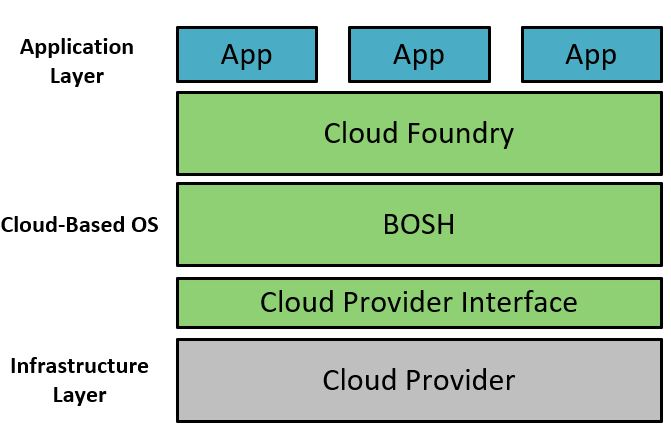
\includegraphics[width=10cm]{img/Cloud_Foundry_Layers.JPG}
		\caption[Einordnung Cloud Foundry Plattform]{Einordnung Cloud Foundry Plattform\\
			(\cite[Eigene Abbildung in Anlehnung an][S. 9]{Winn.2017})}
		\label{Cloud_Foundry_Layers}
	\end{center}
\end{figure}
\\
Wie aus der Grafik \ref{Cloud_Foundry_Layers} entnommen werden kann, bezeichnet Duncan Winn \ac{CF} als Teil eines Cloud basierten Betriebssystems. Dieses Betriebssystem verbirgt die eigentlichen Rechenressourcen, wie beispielsweise den virtuellen Speicher, den Arbeitsspeicher und die \acsp{CPU} und abstrahiert diese für den Endbenutzer in einfach verwendbare Dienste.\autocite[Vgl.][S. 8]{Winn.2017}\\
BOSH ist ein Open-Source Tool zur automatisierten Bereitstellung von Software und übernimmt das Management des Softwarelebenszyklus. Dabei wird mittels Manifestdateien die Provisionierung der virtuellen Maschinen, die Überwachung der Softwarekomponenten sowie die Anwendungsaktualisierungen mit \textbf{Zero-to-minimal Downtime} ermöglicht. \\
Die Erläuterung des Begriffs Zero-to-minimal Downtime erfolgt in Kapitel \ref{bewertung_cf}.\\
Mit Hilfe der einheitlich definierten Manifestdateien ermöglicht BOSH eine von der Infrastruktur unabhängige Beschreibung der Anwendungsbereitstellung.\autocite[Vgl.][S. 14-15]{Winn.2017}
\\
Zudem gehört \ac{CF} zur Cloud Foundry Foundation, welche eine Non-Profit-Organisation ist und ihre Produkte unter der freien Open-Source-Softwarelizenz Apache 2.0 veröffentlicht.\autocite[Vgl.][]{GitHubRepositoryCloudFoundry.2020}
%Laut Duncan Winn sind generelle cloud-native PaaS-Lösungen und somit auch \ac{CF} rechthaberisch. Das bedeutet, dass native Services der Plattform auf Best Practices basieren. Dadurch sind diese klar definiert und somit auch in ihrer Funktionsweise eingeschränkt. , wie beispielsweise die das Deployen von Microservices erfolgen soll. Dadurch soll eine einheitliche Benutzererfahrung unabhängig von der verwendeten Infrastruktur ermöglicht werden. \autocite[Vgl.][ 1. - The Opinionated Platform]{Winn.2017} \\

\section{Virtualisierung der Infrastruktur}
\subsection{Abgrenzung von Containern zu virtuellen Maschinen}
Generell verfolgen sowohl virtuelle Maschinen als auch Containertechnologien die Isolation einzelner Softwarekomponenten auf einem physischen Rechner. \autocite[Vgl.][S. 32-33]{Oggl.2018}
Dabei basieren laut Oliver Liebel fast alle Containertechnologien auf den Isolationsmechanismen des Linux Kernels, den \textbf{Linux Kernel Namespaces}. Dabei wird beispielsweise der PID-Namespace zur Kapselung der Container-Prozesse in eigenständige Root-Prozessbäume innerhalb des eigentlichen Host-Prozessbaumes verwendet.\autocite[Vgl.][S. 80-81]{Liebel.2019}
\\
\begin{figure}[h]
	\begin{center}
		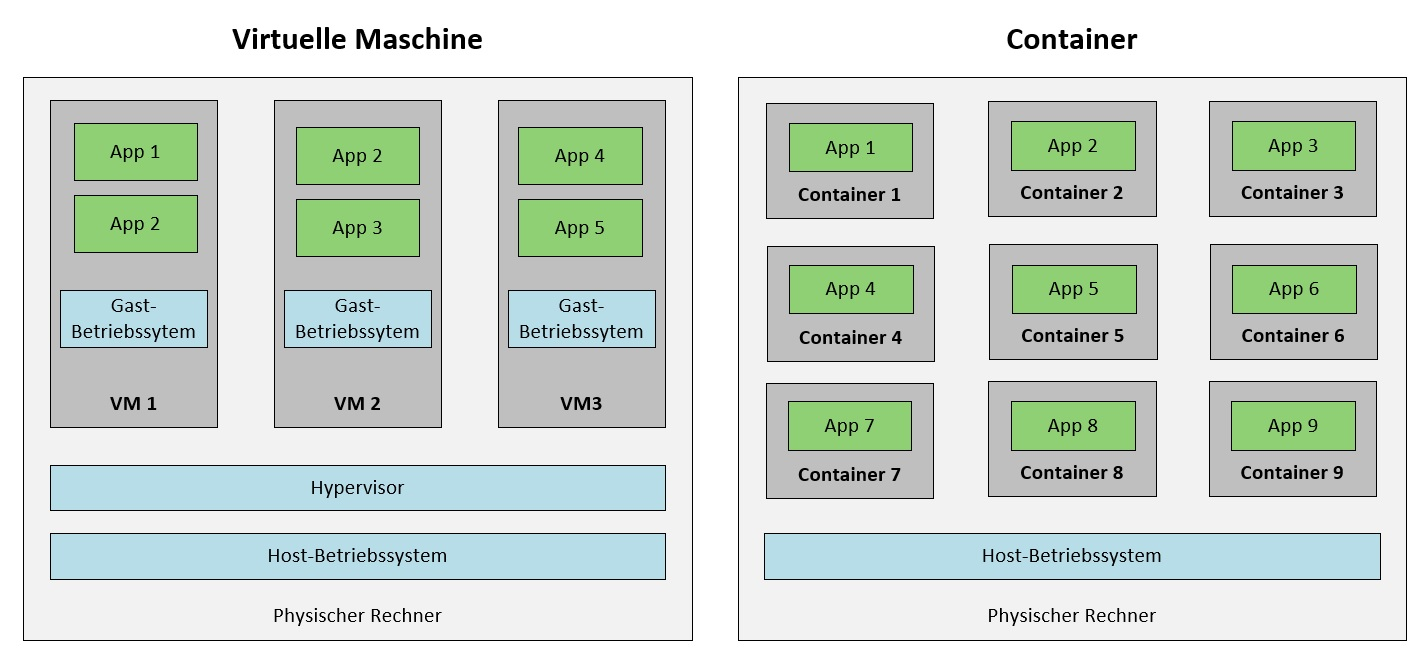
\includegraphics[width=16cm]{img/VM_vs_Container.JPG}
		\caption[Vergleich der Anwendungsbereitstellung mit \acsp{VM} und Containern]{Vergleich der Anwendungsbereitstellung mit \acsp{VM} und Containern\\
			(\cite[Eigene Abbildung in Anlehnung an][S.11]{Luksa.2018})}
		\label{Vergleich_VM_Container}
	\end{center}
\end{figure}
\newpage
Wie der Abbildung \ref{Vergleich_VM_Container} entnommen werden kann, haben Container im Vergleich zu \acsp{VM} kein eigenes Gast-Betriebssystem, sondern sind isolierte Prozesse, die auf dem Betriebssystem des zugrundeliegenden Hosts laufen. Dadurch können die bei \acsp{VM} benötigten Systemprozesse eingespart und Hardwareressourcen des physischen Rechners effektiver genutzt werden.\autocite[Vgl.][S. 10-12]{Luksa.2018}
\subsection{Containerisierung mit Docker}
\textbf{Docker} ist eine Container-Engine-Plattform und ermöglicht das ``Verpacken, Verteilen und Ausführen von Anwendungen`` \autocite[][S. 15]{Luksa.2018} mittels \textbf{Docker-Images}. Hierbei können die Images in einer zentralen \textbf{Image Registry} abgelegt werden. Dies ermöglicht die generelle Portierung der Container auf beliebige physische Rechner. Die einzige Voraussetzung hierfür ist, dass auf dem Host-Rechner die für das Docker Image vorgesehene Linux-Kernel Version läuft. Außerdem dienen die Images als Grundlage für die Container. Ein Container ist ein in einem ressourceneingeschränkten und isolierten Prozess des Host-Rechners ausgeführtes Image. \autocite[Vgl.][S. 14-15, 18]{Luksa.2018} Eine alternative Container Engine ist beispielsweise \textbf{cri-o}.\autocite[Vgl.][S. 79]{Liebel.2019}%Wie in Abbildung \ref{Container_Schichten_Architektur} zu sehen ist, gibt es neben Docker weitere alternative Container Engines, wie beispielsweise \textbf{cri-o}.\autocite[Vgl.][S. 108]{Liebel.2019} %Container-Engine, welche die \ac{OCI}-Standards erfüllt.\autocite[Vgl.][S. 108]{Liebel.2019}
\\
\begin{figure}[h]
	\begin{center}
		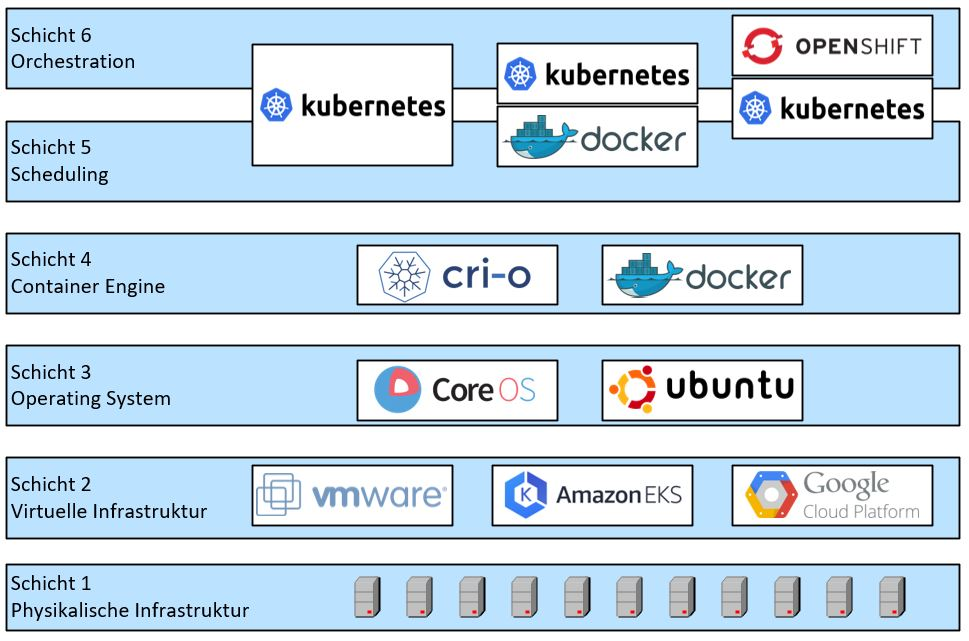
\includegraphics[width=14cm]{img/Container_Schichten_Architektur.JPG}
		\caption[Schichten einer containerbasierten Anwendungsbereitstellung]{Schichten einer containerbasierten Anwendungsbereitstellung\\
			(\cite[Eigene Abbildung in Anlehnung an][S.79]{Liebel.2019})}
		\label{Container_Schichten_Architektur}
	\end{center}
\end{figure}
\newpage
\section{Kubernetes}
\label{Kubernetes}
Kubernetes ist ein Open Source Softwaresystem zur Bereitstellung, Verwaltung und Orchestration von containerbasierten Anwendungen. Dabei wird die Hardwareschicht der Infrastruktur auf \textbf{Nodes} abstrahiert. Für das Entwicklungs- und Betriebsteam stellt sich das gesamte Infrastruktursystem, das physisch aus mehreren Rechnerclustern bestehen kann, als einziges virtuelles System dar. Dadurch sollen sich die Entwickler auf die eigentliche Anwendungsentwicklung konzentrieren können, indem sie auf die von Kubernetes bereitgestellten Dienste zurückgreifen können. Dies sind exemplarisch native Funktionen zur Lokalisierung von Services, automatischen Skalierung der Bereitstellungen, Lastenausgleichsfunktionen sowie Selbstheilungsmechanismen für die bereitgestellten Anwendungen.\autocite[Vgl.][S. 19-21]{Luksa.2018}\\
Bei der Kubernetes Plattform werden die Docker Container innerhalb von \textbf{Pods} bereitgestellt. Hierbei sind Pods generell die kleinste möglichste Recheneinheit, welche auf einem Kubernetes Cluster bereitgestellt werden kann und prinzipiell aus einem oder mehreren Containern bestehen können.
Zudem ist zu beachten, dass die in einem Pod ausgeführten Container im gleichen Kontext und dadurch mit einem geteilten Speicher und dem gleichen Netzwerk bereitgestellt werden. Damit teilen sich diese Container auch die gleiche \ac{IP}-Adresse und denselben Portraum.\\
Generell dienen die Kubernetes Pods als Abstraktionsmedium für die Bereitstellung von entweder eng oder lose gekoppelter Container. Dabei können eng gekoppelte Container innerhalb von einem Pod und lose gekoppelte Container in unterschiedlichen Pods bereitgestellt werden.\autocite[Vgl.][What is a Pod, Motivation for Pods]{KubernetesAuthors.20190806}
\subsection{Grundlagen des Kubernetes Clusters}
\label{Grundlagen_Kubernetes}
Generell besteht ein Kubernetes Cluster aus mindestens einer \textbf{Master Node} und einer \textbf{Worker Node}.\\
Dabei werden vereinfacht betrachtet die aus der Abbildung \ref{Grafik_Grundlagen_Kubernetes_Cluster} zu entnehmenden Komponenten auf der Master und Worker Node des Kubernetes Clusters bereitgestellt.
\\
\begin{figure}[h]
	\begin{center}
		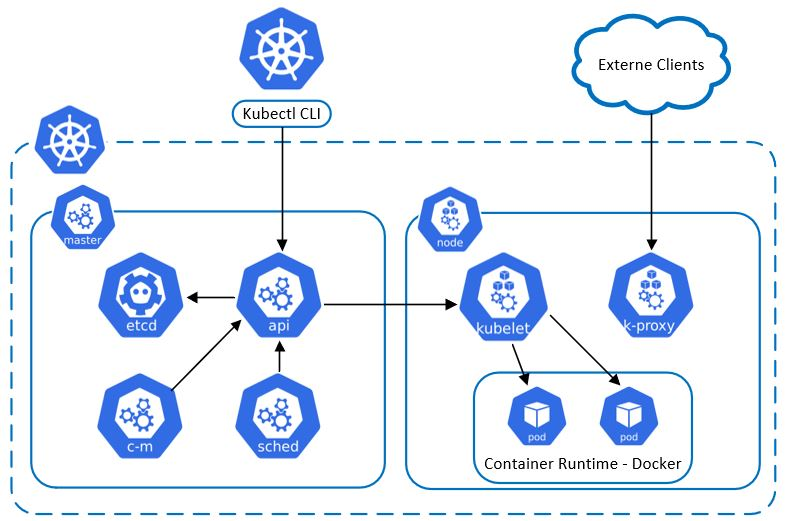
\includegraphics[width=16cm]{img/Kubernetes_Aufbau.JPG}
		\caption[Grundlagen Kubernetes Cluster]{Grundlagen Kubernetes Cluster \\
			(\cite[Eigene Abbildung in Anlehnung an][S.563]{Liebel.2019})}
		\label{Grafik_Grundlagen_Kubernetes_Cluster}
	\end{center}
\end{figure}
\\
\newpage
\begin{description}
	\item[API-Server] \hfill \\
	Der \ac{API}-Server ist die zentrale Administrationskomponente zur Verwaltung der Clusterobjekte. Dabei nimmt er alle Anfragen an, die zum Beispiel mit der \textbf{kubectl}-\ac{CLI} oder anderer \ac{GUI}-Lösungen an die \ac{REST}-Schnittstelle des \ac{API}-Servers gesendet werden. Anschließend validiert und verarbeitet er diese. Des Weiteren beinhaltet er alle Definitionen der Kubernetes-Objekte und stellt diese bereit.\autocite[Vgl.][S. 564-565]{Liebel.2019}
	\item[Controller Manager] \hfill \\
	Der Controller Manager übernimmt clusterweite Aufgaben, wie etwa die Sicherstellung der definierten Anzahl an replizierten Pods, die Überwachung der Worker Nodes sowie Gegenmaßnahmen bei einem Ausfall einer Node.\autocite[Vgl.][S. 565]{Liebel.2019}
	\item[Scheduler] \hfill \\
	Der Scheduler ist zuständig für die Zuweisung der Pod-Instanzen auf die Worker Nodes. Hierbei versucht er die aktuellen Workloads der Worker Nodes mittels deren freien Ressourcenkapazitäten zu optimieren. \autocite[Vgl.][S. 566]{Liebel.2019}
	\item[etcd] \hfill \\
	Der zentrale Key-Value Store etcd dient der persistenten Sicherung der Clusterkonfigurationen und des aktuellen Zustandes des \ac{API}-Servers.
	\item[kubelet] \hfill \\
	Der kubelet-Service fungiert als Kommunikations- und Steuerungsschnittstelle der \textbf{Worker Nodes} für den API-Server. Dabei sorgt er für die Bereitstellung der Kubernetes-Objekte in der lokalen Container Runtime, wie beispielsweise der Docker Engine.\autocite[Vgl.][S. 566-567]{Liebel.2019}
	\item[kube-proxy] \hfill \\
	Der kube-proxy-Dienst kümmert sich um die ``clusterweite, interne Bereitstellung von Services […] und um die Annahmen und Weiterleitung von der Außenwelt eingehender Requests``.\autocite[][S. 568]{Liebel.2019}
\end{description}
Die Erläuterung der einzelnen Kubernetes-Objekte, welche innerhalb des Prototyps verwendet und implementiert werden, erfolgt in den Kapiteln \ref{Konzeption_K8s_Cluster} und \ref{Umsetzung_K8s_Cluster}.\\
\subsection{Cluster Verwaltung mittels Gardener}
\label{Cluster_Verwaltung}
Das Gardener Projekt ist ein Open Source Projekt, welches das Ziel der kostenfreien Provisionierung von Kubernetes Clustern as-a-Service verfolgt. Dabei können die Kubernetes Cluster mit Hilfe von Gardener in wenigen Schritten konfiguriert und provisioniert werden. Für die weitere Verwaltung des Kubernetes Clusters bietet Gardener ein Dashboard sowie bereits vorinstallierte Lösungen und Tools welche beispielsweise für das Monitoring der Kubernetes Master Nodes eingesetzt werden können.\autocite[Vgl.][Gardener Dashboard]{GardenerAuthors.20200120}
\\
Zudem unterstützt Gardener den Multi-Cloud Ansatz dadurch, dass die benötigte Infrastruktur von unterschiedlichen \ac{IaaS}-Providern aus weltweit verteilten Regionen verwendet werden kann. Hierbei können zum aktuellen Zeitpunkt der vorliegenden Thesis die folgenden \ac{IaaS}-Provider eingesetzt werden: \ac{AWS}, Microsoft Azure Cloud, \ac{GCP}, Open Stack und Alibaba Cloud.\autocite[Vgl.][K8s Conformance Test Coverage]{GardenerAuthors.20200121} Die Auswahl der Regionen ist hierbei vom \ac{IaaS}-Provider abhängig.\\
Für die technische Bereitstellung des Kubernetes Clusters wird ausschließlich Rechenkapazität in Form von virtuellen Maschineninstanzen und persistentem Speicherplatz benötigt.\\
Des Weiteren ermöglicht Gardener eine automatische Skalierung der für die Nodes verwendeten \acsp{VM}.
\newpage 
Dabei definiert der Clusteradministrator den Maschinentyp der virtuellen Recheninstanzen, die Art des persistenten Speichermediums sowie die minimale und maximale Anzahl an Recheninstanzen. Die horizontale Skalierung wird anschließend automatisch abhängig vom Rechenkapazitätsbedarf des Kubernetes Clusters durchgeführt. \\
Außerdem stellt Gardener verglichen mit anderen Cluster-as-a-Service-Anbieter homogene und nicht proprietäre Kubernetes Cluster zur Verfügung. Das bedeutet, dass Gardener durch die Open Source Community versucht einen offenen Standard für die Provisionierung eines Kubernetes Clusters zu etablieren. Allerdings unterstützt Gardener zum Zeitpunkt der vorliegenden Thesis ausschließlich die Container Engine Docker.\\
%Anmerkung: Quelle einfügen!
Eine weitere Funktion, die zur generellen Senkung der Betriebskosten des Clusters genutzt werden kann, ist die Konfiguration des Cluster-Lifecycles. Dabei kann definiert werden, an welchen Tagen und zu welcher Uhrzeit das Cluster automatisch gestartet und wieder heruntergefahren werden soll.\autocite[Vgl.][Configuration]{GardenerAuthors.20200120}
\\
\section{SAP Subscription Billing}
\subsection{Fachliches Anwendungsgebiet}
SAP Subscription Billing ist eine \ac{SaaS}-Lösung zur Automatisierung und Optimierung der Abrechnungs- und Bestellprozesse. Dadurch sollen besonders innovative Geschäftsmodelle, die auf wiederkehrenden Zahlungen oder einer nutzungsabhängigen Gebührenberechnung basieren, schnell geplant, modelliert und umgesetzt werden können.\\ 
Insbesondere durch das nutzungsbasierte Abrechnungsmodell ermöglicht die Softwarelösung ihren Kunden beliebige ``as-a-Service``-Szenarien zu bedienen.
Hierbei sind die von einem Unternehmen angebotenen Produkte und die dafür definierten Tarifpläne der Kern der Softwarelösung. Dadurch können mit Hilfe des effektiven Verbrauchs der Kunden und den für das entsprechende Produkt definierten Tarifplänen die nutzungsabhängige Berechnung der Gebühren durchgeführt werden.\autocite[Vgl.][SAP Subscription Billing]{SAPSEodereinSAPKonzernunternehmen.2019}
\\
\newpage
\subsection{Technische Grundlagen}
Aus technischer Sicht ist SAP Subscription Billing laut der deutschsprachigen SAP Anwendergruppe eine mandantenfähige Softwarelösung, die für den Endanwender in der Public Cloud bereitgestellt wird. Generell basiert die Softwareösung auf einer Microservice-Architektur, welche mittels der \ac{CF}-Umgebung der \ac{SCP} bereitgestellt wird. Zudem bietet die Lösung offene \ac{API}-Schnittstellen an, welche zur Integration in eigene Infrastruktur-Landschaften genutzt werden können. Alternativ ist die Lösung mittels des zentralen Einstiegspunktes \url{https://revenue.cloud.sap} auch als Webanwendung mit einer grafischen Benutzeroberfläche erreichbar. \autocite[Vgl.][]{DeutschsprachigeSAPAnwendergruppe.2018}\\
Des Weiteren wurde die \ac{SaaS}-Lösung mit den zur Verfügung stehenden \acsp{API}\footnote{\ac{API} Hub SAP Subscription Billing: \url{https://api.sap.com/package/SAPHybrisRevenueCloud?section=Artifacts}} in weitere SAP Lösungen, wie beispielsweise SAP S/4HANA Cloud oder SAP Commerce Cloud integriert.\autocite[Vgl.][SAP Subscription Billing - Integration]{SAPSEodereinSAPKonzernunternehmen.20200205} Die ausführliche Erläuterung des technischen Aufbaus der \ac{SaaS}-Lösung erfolgt in Kapitel \ref{technischer_aufbau_cf}.\\


